\renewcommand{\prechaptername}{付録}
\renewcommand{\postchaptername}{}
\renewcommand{\thechapter}{\Alph{chapter}}
\setcounter{chapter}{0}

\chapter{タイミング分布}
\thispagestyle{empty}
\label{app:app1}
TGC~検出器のタイミング較正におけるすべてのチェンバーの結果を記す。

    \begin{figure}[htbp]
		\centering
		\begin{tabular}{l}
			\begin{minipage}{0.22\hsize}
				\includegraphics[width=\textwidth,page=2]{img/pdf5/master_timingplot_comp.pdf}
			\end{minipage}
			
			\begin{minipage}{0.22\hsize}
				\includegraphics[width=\textwidth,page=4]{img/pdf5/master_timingplot_comp.pdf}
			\end{minipage}

			\begin{minipage}{0.22\hsize}
				\includegraphics[width=\textwidth,page=6]{img/pdf5/master_timingplot_comp.pdf}
			\end{minipage}
			
			\begin{minipage}{0.22\hsize}
				\includegraphics[width=\textwidth,page=8]{img/pdf5/master_timingplot_comp.pdf}
			\end{minipage}\\

			\begin{minipage}{0.22\hsize}
				\includegraphics[width=\textwidth,page=10]{img/pdf5/master_timingplot_comp.pdf}
			\end{minipage}
			\vspace{0.5cm}\\ 

            \begin{minipage}{0.22\hsize}
				\includegraphics[width=\textwidth,page=12]{img/pdf5/master_timingplot_comp.pdf}
			\end{minipage}
			
			\begin{minipage}{0.22\hsize}
				\includegraphics[width=\textwidth,page=14]{img/pdf5/master_timingplot_comp.pdf}
			\end{minipage}

			\begin{minipage}{0.22\hsize}
				\includegraphics[width=\textwidth,page=16]{img/pdf5/master_timingplot_comp.pdf}
			\end{minipage}
			
			\begin{minipage}{0.22\hsize}
				\includegraphics[width=\textwidth,page=18]{img/pdf5/master_timingplot_comp.pdf}
			\end{minipage}\\

			\begin{minipage}{0.22\hsize}
				\includegraphics[width=\textwidth,page=20]{img/pdf5/master_timingplot_comp.pdf}
			\end{minipage}
			
			\begin{minipage}{0.22\hsize}
				\includegraphics[width=\textwidth,page=22]{img/pdf5/master_timingplot_comp.pdf}
			\end{minipage}
			\vspace{0.5cm}\\ 
			
			\begin{minipage}{0.22\hsize}
				\includegraphics[width=\textwidth,page=24]{img/pdf5/master_timingplot_comp.pdf}
			\end{minipage}
			
			\begin{minipage}{0.22\hsize}
				\includegraphics[width=\textwidth,page=26]{img/pdf5/master_timingplot_comp.pdf}
			\end{minipage}

			\begin{minipage}{0.22\hsize}
				\includegraphics[width=\textwidth,page=28]{img/pdf5/master_timingplot_comp.pdf}
			\end{minipage}
			
			\begin{minipage}{0.22\hsize}
				\includegraphics[width=\textwidth,page=30]{img/pdf5/master_timingplot_comp.pdf}
			\end{minipage}\\

			\begin{minipage}{0.22\hsize}
				\includegraphics[width=\textwidth,page=32]{img/pdf5/master_timingplot_comp.pdf}
			\end{minipage}
			
			\begin{minipage}{0.22\hsize}
				\includegraphics[width=\textwidth,page=34]{img/pdf5/master_timingplot_comp.pdf}
			\end{minipage}
			\vspace{0.5cm}\\ 

			\begin{minipage}{0.22\hsize}
				\includegraphics[width=\textwidth,page=36]{img/pdf5/master_timingplot_comp.pdf}
			\end{minipage}
			
			\begin{minipage}{0.22\hsize}
				\includegraphics[width=\textwidth,page=38]{img/pdf5/master_timingplot_comp.pdf}
			\end{minipage}

			\begin{minipage}{0.22\hsize}
				\includegraphics[width=\textwidth,page=40]{img/pdf5/master_timingplot_comp.pdf}
			\end{minipage}
			
			\begin{minipage}{0.22\hsize}
				\includegraphics[width=\textwidth,page=42]{img/pdf5/master_timingplot_comp.pdf}
			\end{minipage}
			\vspace{0.5cm}\\ 

		\end{tabular}
		\caption[wire~チャンネルにおけるタイミングパラメータを用いた~TGC~の評価。]{wire~チャンネルにおけるタイミングパラメータを用いた~TGC~の評価。橙色(■)、緑色(●)、青色(▲)はそれぞれRun~2~データ、改良後のシミュレーション、改良前のシミュレーションを表している。各プロットにチェンバーの名称を示している。}
		\label{fig:timingPlotCompWire}
	\end{figure}
    
    \begin{figure}[htbp]
		\centering
		\begin{tabular}{l}
			\begin{minipage}{0.22\hsize}
				\includegraphics[width=\textwidth,page=3]{img/pdf5/master_timingplot_comp.pdf}
			\end{minipage}
			
			\begin{minipage}{0.22\hsize}
				\includegraphics[width=\textwidth,page=5]{img/pdf5/master_timingplot_comp.pdf}
			\end{minipage}

			\begin{minipage}{0.22\hsize}
				\includegraphics[width=\textwidth,page=7]{img/pdf5/master_timingplot_comp.pdf}
			\end{minipage}
			
			\begin{minipage}{0.22\hsize}
				\includegraphics[width=\textwidth,page=9]{img/pdf5/master_timingplot_comp.pdf}
			\end{minipage}\\

			\begin{minipage}{0.22\hsize}
				\includegraphics[width=\textwidth,page=11]{img/pdf5/master_timingplot_comp.pdf}
			\end{minipage}
			\vspace{0.5cm}\\ 

            \begin{minipage}{0.22\hsize}
				\includegraphics[width=\textwidth,page=13]{img/pdf5/master_timingplot_comp.pdf}
			\end{minipage}
			
			\begin{minipage}{0.22\hsize}
				\includegraphics[width=\textwidth,page=15]{img/pdf5/master_timingplot_comp.pdf}
			\end{minipage}

			\begin{minipage}{0.22\hsize}
				\includegraphics[width=\textwidth,page=17]{img/pdf5/master_timingplot_comp.pdf}
			\end{minipage}
			
			\begin{minipage}{0.22\hsize}
				\includegraphics[width=\textwidth,page=19]{img/pdf5/master_timingplot_comp.pdf}
			\end{minipage}\\

			\begin{minipage}{0.22\hsize}
				\includegraphics[width=\textwidth,page=21]{img/pdf5/master_timingplot_comp.pdf}
			\end{minipage}
			
			\begin{minipage}{0.22\hsize}
				\includegraphics[width=\textwidth,page=23]{img/pdf5/master_timingplot_comp.pdf}
			\end{minipage}
			\vspace{0.5cm}\\ 
			
			\begin{minipage}{0.22\hsize}
				\includegraphics[width=\textwidth,page=25]{img/pdf5/master_timingplot_comp.pdf}
			\end{minipage}
			
			\begin{minipage}{0.22\hsize}
				\includegraphics[width=\textwidth,page=27]{img/pdf5/master_timingplot_comp.pdf}
			\end{minipage}

			\begin{minipage}{0.22\hsize}
				\includegraphics[width=\textwidth,page=29]{img/pdf5/master_timingplot_comp.pdf}
			\end{minipage}
			
			\begin{minipage}{0.22\hsize}
				\includegraphics[width=\textwidth,page=31]{img/pdf5/master_timingplot_comp.pdf}
			\end{minipage}\\

			\begin{minipage}{0.22\hsize}
				\includegraphics[width=\textwidth,page=33]{img/pdf5/master_timingplot_comp.pdf}
			\end{minipage}
			
			\begin{minipage}{0.22\hsize}
				\includegraphics[width=\textwidth,page=35]{img/pdf5/master_timingplot_comp.pdf}
			\end{minipage}
			\vspace{0.5cm}\\ 

			\begin{minipage}{0.22\hsize}
				\includegraphics[width=\textwidth,page=37]{img/pdf5/master_timingplot_comp.pdf}
			\end{minipage}
			
			\begin{minipage}{0.22\hsize}
				\includegraphics[width=\textwidth,page=39]{img/pdf5/master_timingplot_comp.pdf}
			\end{minipage}

			\begin{minipage}{0.22\hsize}
				\includegraphics[width=\textwidth,page=41]{img/pdf5/master_timingplot_comp.pdf}
			\end{minipage}
			
			\begin{minipage}{0.22\hsize}
				\includegraphics[width=\textwidth,page=43]{img/pdf5/master_timingplot_comp.pdf}
			\end{minipage}
			\vspace{0.5cm}\\ 

		\end{tabular}
		\caption[strip~チャンネルにおけるタイミングパラメータを用いた~TGC~の評価。]{strip~チャンネルにおけるタイミングパラメータを用いた~TGC~の評価。橙色(■)、緑色(●)、青色(▲)はそれぞれRun~2~データ、改良後のシミュレーション、改良前のシミュレーションを表している。各プロットにチェンバーの名称を示している。}
		\label{fig:timingPlotCompStrip}
	\end{figure}
	